%\documentclass{article}
%\usepackage[utf8]{inputenc}
%\usepackage[russian]{babel}
%\usepackage{multicol}
%\usepackage[left=10mm, top=5mm, right=15mm,bottom=0mm]{geometry}
%\usepackage{multicol}
%\usepackage{multirow}
%\usepackage{graphicx}
%\begin{document}

\pagestyle{empty}

\begin{center}
\scriptsize{\qquad \qquad \qquad \qquad \quad \qquad \qquad \qquad \qquad \qquad ГИПОТЕЗА ТАНИЯМЫ И ПОСЛЕДНЯЯ ТЕОРЕМА ФЕРМА \qquad \qquad \qquad \qquad \qquad \qquad \qquad \qquad \qquad } \large{\textit{5}}
\end{center}
\begin{multicols}{3}

\begin{left}
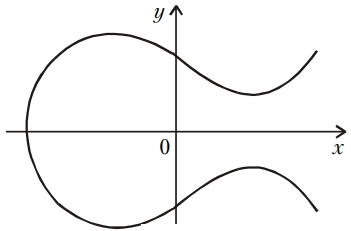
\includegraphics[scale=0.5]{image1}
\end{left}
\begin{left}
\par Рис. 4 
\par 
\end{left}
\begin{left}
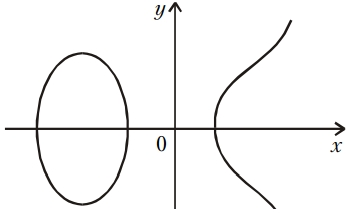
\includegraphics[scale=0.5]{image2}
\end{left}
\begin{left}
\par Рис. 5 
\par
\end{left}

Для кривой, заданной в канонической форме (2), дискриминант $\Delta$ определяется формулой \[\Delta = -(4a^3+27b^2).\] Пусть E - некоторая эллиптическая кривая, заданная уравнением \[y^2 = x^3+ax+b,\] в котором a и b - целые числа. Для простого числа p рассмотрим сравнение \[y^2 \equiv x^3+\overline ax+\overline b (mod\: p), \qquad (3)\] где $\overline a$ и $\overline b$ - остатки от деления целых чисел a и b на p, и обозначим через $n_p$ число решений этого сравнения. Числа $n_p$ очень полезны при исследовании вопроса о разрешимости уравнений вида (2) в целых числах: если какое-то $n_p$ равно нулю, то уравнение (2) не имеет целочисленных решений. Однако вычислить числа $n_p$ удается лишь в редчайших случаях. В то же время известно, что $|p-n_p| \leq 2\sqrt{p}$ (теорема Хассе).\par Рассмотрим те простые числа p, которые делят дискриминант $\Delta$ эллиптической кривой (2). Можно доказать, что для таких p многочлен $x^3+\overline a x + \overline b$ можно записать одним из двух способов: \[x^3+\overline a x+\overline b \equiv (x+\overline \alpha)^2(x+\overline \beta)(mod\:p)\]или \[x^3+\overline a x+\overline b \equiv (x+\overline \gamma)^3(mod\:p),\] где $\overline \alpha$, $\overline \beta$, $\overline \gamma$ - некоторые остатки от деления на p. Если для всех простых p, делящих дискриминант кривой, реализуется первая из двух указанных возможностей, то эллиптическая кривая  называется \textit{полустабильной}.\parПростые числа, делящие дискриминант, можно объединить в так называемый \textit{кондуктор} эллиптической кривой. Если \textit{E} - полустабильная кривая, то её кондуктор \textit{N} задаётся формулой \[\qquad \qquad \quad \quad N=\prod_{p|\Delta} p^\varepsilon_p \:,\qquad \qquad (4)\] где для всех простых чисел $p \geq 5$, делящих $\Delta$, показатель $\varepsilon_p$ равен 1. Показатели $\varepsilon_2$ и $\varepsilon_3$ вычисляются с помощью специального алгоритма.\section*{Модулярные формы и молекулярные эллиптические кривые} Обозначим через \textit{H} верхнюю комплексную полуплоскость. Пусть \textit{N} - натуральное и k - целое числа. \textit{Модулярной параболической формой веса k} уровня N называется аналитическая функция f(z), заданная в верхней полуплоскости и удовлетворяющая соотношению \[ \qquad f(\frac{az+b}{cz+d}) = (cz+d)^kf(z) \qquad(5)\] для любых целых a, b, c, d таких, что $ad-bc=1$ и c делится на N. Кроме того, предполагается, что\[\lim_{t \to\\+0} f(r+it) = 0,\]где r - рациональное число, и что \[\lim_{t\to\infty} f(it) = 0.\] Пространство модулярных параболических форм веса k уровня N обозначается через $S_k(N)$. Можно показать, что оно имеет конечную размерность.\parВ дальнейшем нас будут особо интересовать модулярные параболические формы веса 2. Для малых N размерность dim $S_2(N)$ пространства $S_2(N)$ представлена в таблице: 
\begin{center}
\begin{tabular}{|c|c|c|c|c|c|c|}
\hline
$N<10$ & 11 & 12 & 13 & 14 & 15 & 16 \\ \hline
0 & 1 & 0 & 0 & 1 & 1 & 0 \\ \hline
\multirow{3}{*}{ \qquad } & 17 & 18 & 19 & 20 & 21 & 22 \\
\cline{2-7}
            & 1 & 0 & 1 & 1 & 1 & 2 \\
\hline
\end{tabular}
\end{center}
 \par В частности, \[ \qquad \qquad \qquad \quad dim \; S_2(2) = 0. \qquad \quad (6)\] \par Отметим, что эта нехитрая формула сыграет важную роль в доказательстве теоремы Ферма. \par Из условия (5) следует, что $f(z + 1) = f(z)$ для каждой формы $f \in S_2(N).$ Стало быть, $f$ является периодической функцией. Такую функцию можно представить в виде \[\qquad \qquad f(z) = \sum_{n=1}^{\infty} a_n q^n, q = e^{2\pi i z}.  \quad (7)\] \par Назовём модулярную параболическую форму $f(z) \in S_2(N)$ \textit{собственной, если её коэффициенты - целые числа, удовлетворяющие соотношениям} \[a_1 
 = 1; \] $a_{p^r},a_p = a_{p^{r+1}}pc_{p^{r-1}}$ для простого p,\par \qquad  \qquad  не делящего число \textit{N}; \:\: (8) \[a_p^r=(a_p)^r\] \qquad \qquad для простого p, \par \qquad \qquad \qquad \quad делящего число N; \[a_mn=a_ma_n, если (m, n) = 1.\] \par Сформулируем теперь определение, играющее ключевую роль в доказательстве теоремы Ферма. Эллиптическая кривая с рациональными коэффициентами и кондуктором N называется \textit{модулярной}, если найдётся такая собственная форма. \[ \qquad \quad f(z) = \sum_{n=1}^{\infty} a_n q^n \in S_2(N), \qquad (9).\] что $a_p = p - n_p$ для почти всех простых чисел p. Здесь $n_p$ - число решений сравнения (3). \section*{\qquad Гипотеза Таниямы} Определение модулярной эллиптической кривой является настолько жёстким, что на первый взгляд кажется невероятным существование хотя бы одной такой кривой. Трудно представить, что функция $f(z),$ удовлетворяющая перечисленным выше весьма ограничительным условиям (5) и (8), разлагается в ряд (7), коэффициенты которого связаны с практически невычислимыми числами $n_p$. Однако эмпирический материал, полученный в первой по-
\end{multicols}
\scriptsize{2 Квант №4}
%\end{document}
